\begin{frame}
    \frametitle{``Lisp in C's Clothing'' \citep{crockford2001javascript}}
    \itemize{
        \item{\textbf{Dynamically Typed:} no static type annotations or type
              checks.}
        \item{\textbf{C-Like Syntax:} curly-braces, \texttt{for}, semicolons,
              dot operator.}
        \item{\textbf{Object-Oriented:} OOP patterns, properties, inheritance
              (prototypal, not class-based).}
        \item{\textbf{Functional:} FP patterns, function literals, closures with
              lexical scoping.}
    }
\end{frame}

\begin{frame}
    \frametitle{``Programming languages that influenced JavaScript''
                \citep{rauschmayer2014speaking}}
    \begin{figure}
        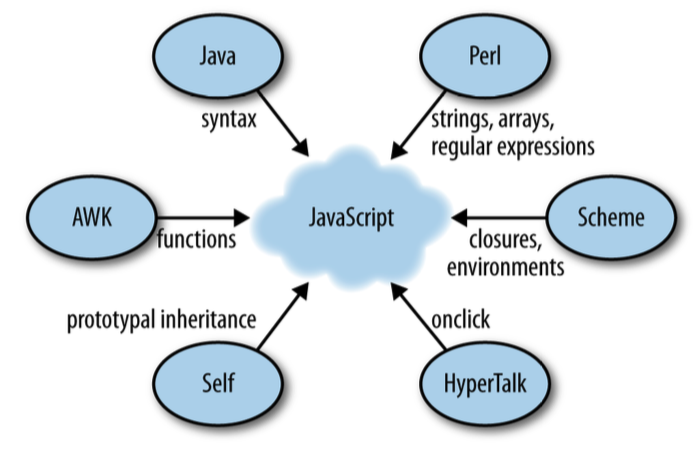
\includegraphics[scale=0.35]{influences}
    \end{figure}
\end{frame}

\begin{frame}
    \frametitle{Problem and Goal}
    \begin{itemize}
        \item{\textbf{Problem:} Though JS may syntactically look similar to
              other languages, many may find the language's semantics
              surprising.}
        \item{\textbf{Goal:} Present a few of these to promote awareness.}
    \end{itemize}
\end{frame}

\begin{frame}[fragile]
    \frametitle{A Surprising Example}
    What is going on here?
    \begin{lstlisting}[language=JavaScript]
    function f() {
        x = new Object();
    }
    f()
    window.x === x && x === this.x  // true?!
    \end{lstlisting}
    \texttt{x} is a variable, but somehow we can access it in 3 syntactically
    distinct ways. Here, we can see that \texttt{window}, the unique global
    object, is:
    \begin{itemize}
        \item{An object by which \textit{variables} are accessed.}
        \item{An object by which \textit{properties} are accessed.}
        \item{An object produced by the \lstinline{this} keyword.}
    \end{itemize}
\end{frame}
